


%%%%%%%%                       02 - Cíle práce                      %%%%%%%%
%---------------------------------------------------------------------------
% Stručně uveďte cíle Vaší práce.
% Vhodné jsou max. 3 odrážky/věty s hlavními cíli.

% Někdy je motivace totožná s formulací cílů. Nenuťte se do dvou slajdů, když je správnější myšlenku vyjádřit jedním... 

% Formulujte, co je cílem:
%  - Jak se pozná úspěšný výsledek?
%  - Co jsou výstupy?
%  - Jaké vlastnosti má mít úspěšný výsledek?
%  - Kde to půjde použít?

% Lepší je bez použití odrážek:
%  - mít dostatečně dobrý obrázek, který budete svými slovy komentovat 
%  - na obrázku je vizuální sdělení, sdělení slovní dodáte pusou

% Je zbytečné říkat generická a obecná tvrzení: "Řešení by mělo být rychlé, spolehlivé a robustní" - toto jsou obecné požadavky na cokoli a informační hodnota sdělení je NULA - je to jen plýtvání časem a inteligencí.
% Mluvte konkrétně: Jaké konkrétní vlastnosti má mít Vaše řešení, co konkrétně znamená "robustní", co konkrétně znamená "spolehlivé"?

\begin{frame}
  \frametitle{Cíle práce}

  \vspace{-0.2cm}
  \begin{center}
    {\Large \textbf{Fine-tuning LLMs pro řešení matematických úloh}}
  \end{center}

  \vspace{0.2cm}
  \begin{center}
    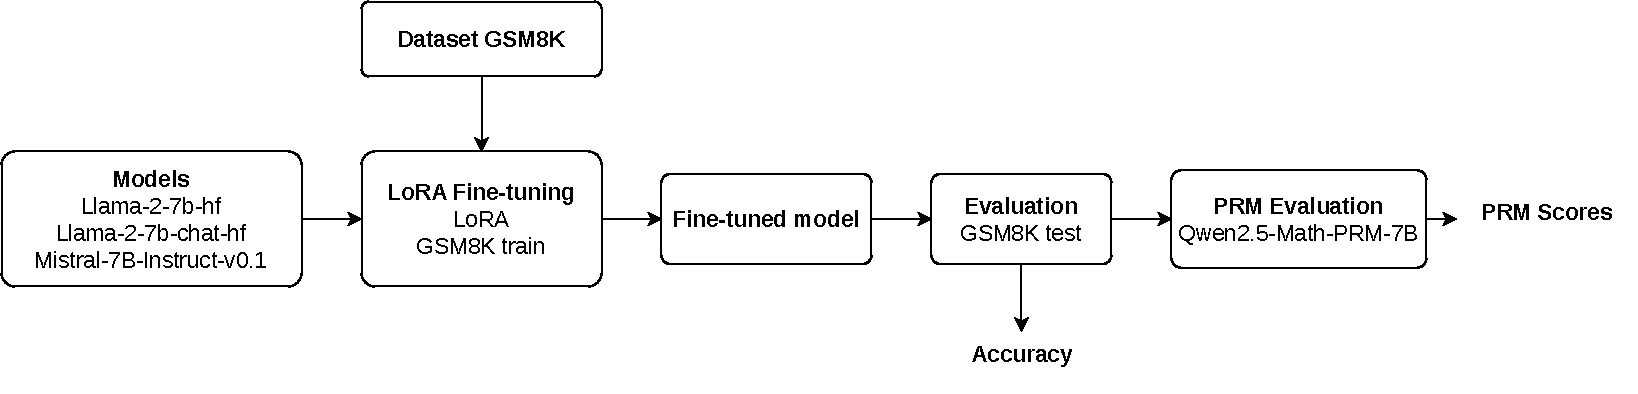
\includegraphics[width=1.03\textwidth]{img/Pipeline.drawio.pdf}
  \end{center}

\end{frame}



%%%%%%%%                  03 - Informace o řešení                   %%%%%%%%
%---------------------------------------------------------------------------
% Cílem  obhajoby je podat zprávu o stavu projektu, nikoliv tedy držet přednášku na zadané téma. Mluvte o tom, co vy jste udělali, jaké jsou vaše výsledky. Mějte na slajdech formální pojmy, buďte přesní, definujte a odkazujte se.

% Prezentace nemusí a vlastně nemá obsahovat:
% -- Výklad použitých algoritmů apod. To patří do přednášky na dané téma, v prezentaci o stavu jen známé algoritmy uveďte podle jména, neznámé algoritmy třeba trochu přibližte, aby bylo zřejmo, o co jde, ale nevysvětlujte je podrobně. Není cílem, aby vaši posluchači algoritmu rozuměli a dokázali ho naprogramovat, ale aby měli představu, na čem pracujete a jak se vám to daří.
% -- Podrobnosti návrhu vašeho systému. Opět, posluchači nebudou váš systém hackovat, nepotřebují detailní strukturu tříd, názvy funkcí, jména souborů, datové formáty apod. Tyto věci uvádějte pouze v takové míře, která pomůže posluchačům udělat si představu, na čem pracujete a jak se vám to daří.

% HEROUT, Adam. Prezentování. Herout.net: Poznámky učitele, kouče, čtenáře. [online]. [cit. 2021-9-15]. Dostupné z: https://www.herout.net/blog/category/prezentovani/
%---------------------------------------------------------------------------

% - Uveďte, jaké zajímavé problémy jste v práci řešili.
% - Mělo by z toho být patrné, že je to závěrečná práce -- ne jen další projekt do předmětu -- tedy je v tom něco netriviálního, zajímavého a přínosného.
% - Raději dva nebo tři slajdy, které ukážete/vysvětlíte během 20 vteřin, než se snažit všechno "namastit" na jeden slajd.
% - Na slajdy je dobré dát vizuální informaci: vzorce, schemata, obrázky, diagramy. Slovní informaci můžete předat pusou. Je dokonale zbytečné a otravné mít na slajdu v odrážkách to samé, co se chystáte říct.
% - Titulek slajdu "Podstatné informace o řešení" je hodně generický. Ve skutečné Vaší prezentaci bude daleko lepší použít specifický titulek na každém ze slajdů, například: "Schéma neuronové sítě pro detekci frňáků", "Návrh nekonečného automatu", "Vytvořená datová sada" apod.

\begin{frame}
\frametitle{Modely}



\begin{columns}[T]

\column{0.32\textwidth}
\begin{block}{Llama-2-7b-hf}
\textbf{Typ:} Base

\textbf{Trénování:}\\
pouze pre-training
\textbf{Velikost:} 7B
\end{block}

\column{0.32\textwidth}
\begin{block}{Llama-2-7b-chat-hf}
\textbf{Typ:} Chat

\textbf{Trénování:}\\
SFT + RLHF

\textbf{Velikost:} 7B
\end{block}

\column{0.32\textwidth}
\begin{block}{Mistral-7B-Instruct}
\textbf{Typ:} Instruct

\textbf{Trénování:}\\
SFT \\
\textbf{Velikost:} 7B
\end{block}

\end{columns}

\vspace{0.6cm}

\centering
$\Downarrow$

\vspace{0.3cm}

\textbf{Hodnoticí model}

\vspace{0.2cm}

\begin{center}
\begin{minipage}{0.55\textwidth}
\begin{block}{Qwen2.5-Math-PRM-7B}
\textbf{Typ:} Process Reward Model \\
\textbf{Účel:} Hodnocení kroků řešení
\end{block}
\end{minipage}
\end{center}

\end{frame}

\begin{frame}
  \frametitle{Dataset}

  % push content up a bit
  

  \textbf{openai/gsm8k}

  \vspace{0.25cm}

  \begin{itemize}
    \item Slovní matematické úlohy
    \item Angličtina
    \item Subset: main
    \item Train: 7\,473 \quad Test: 1\,319
    \item Formát: \texttt{question} + \texttt{answer}
  \end{itemize}

  % space reserved for your dataset example below
  \vspace{0.3cm}

  \begin{block}{Příklad}

\texttt{Question: 'Natalia sold clips to 48 of her friends in April, and then she sold half as many clips in May. How many clips did Natalia sell altogether in April and May?',}\\
\texttt{Answer: 'Natalia sold 48/2 = <<48/2=24>>24 clips in May.\textbackslash nNatalia sold 48+24 = <<48+24=72>>72 clips altogether in April and May.\textbackslash n\#\#\#\# 72'}\\

\end{block}




\end{frame}





%%%%%%%%                    04 - Výsledky práce                     %%%%%%%%
%---------------------------------------------------------------------------
% Shrňte, jakých výsledků se Vám podařilo dosáhnout.
% Uveďte, jakým způsobem byla vyhodnocena funkčnost a správnost řešení.
% Buďte konkrétní: místo "Aplikace je otestovaná", řekněte, kým a jak byla testována, jaké byly výsledky testů.
% Místo "Úspěšnost detektoru je hodně dobrá" řekněte "Úspěšnost detektoru je 93 % mAP" nebo ještě radši ukažte tabulku se srovnáním oproti alternativním řešením.
% Pokud vyhodnocení sestávalo ze dvou nebo tří částí, může být vhodné rozdělit obsah na dva či tři slajdy. Při prezentování je ovšem potřeba se pohlídat, aby čas věnovaný každému slajdu byl adekvátně krátký a nedošlo k přetažení času.

\begin{frame}
    \frametitle{Výsledky práce: Accuracy}

    \begin{table}
      \centering
      \renewcommand{\arraystretch}{1.3}
      \begin{tabular}{lcccc}
        \toprule
        \textbf{Model} & \textbf{Baseline} & \textbf{Fine-tuned} & \textbf{Zlepšení} \\
        \midrule
        Llama-2-7b-hf            & 10.77\% & 33.36\% & \cellcolor{green!20}{+22.6\%} \\
        Llama-2-7b-chat-hf       & 25.47\% & 39.88\% & \cellcolor{green!20}{+14.4\%} \\
        Mistral-7B-Instruct-v0.1 & 42.23\% & 57.01\% & \cellcolor{green!20}{+14.8\%} \\
        \bottomrule
      \end{tabular}
    \end{table}

    \vspace{0.3cm}
    \hrule
    \vspace{0.3cm}

    {\small\textbf{Nejlepší hyperparametry:}}

    \vspace{0.2cm}

    \begin{table}
      \centering
      \small
      \renewcommand{\arraystretch}{1.2}
      \begin{tabular}{lcccc}
    \toprule
    \textbf{Model} & \textbf{lr} & \textbf{r} & \textbf{alpha} \\
    \midrule
    Llama-2-7b-hf            & 3e-4   & 32 & 128 \\
    Llama-2-7b-chat-hf       & 1.5e-4 & 32 & 64  \\
    Mistral-7B-Instruct-v0.1 & 6e-5   & 64 & 128 \\
    \bottomrule
  \end{tabular}
    \end{table}

  \end{frame}

\begin{frame}
\frametitle{Výsledky práce: PRM hodnocení}

\vspace{-0.4cm}

\begin{table}
\centering
\small
\renewcommand{\arraystretch}{1.25}
\begin{tabular}{lccc}
\toprule
\textbf{Model} &
\textbf{avg\_prod} $\uparrow$ &
\textbf{avg\_incorrect} $\downarrow$ &
\textbf{Kroky} \\
\midrule

Llama-2-7b-hf &
0.104 $\to$ \textcolor{green!60!black}{0.269} &
0.051 $\to$ 0.400 &
1417 $\to$  6392 \\

Llama-2-7b-chat-hf &
0.239 $\to$ \textcolor{green!60!black}{0.322} &
0.693 $\to$ \textcolor{green!60!black}{0.443} &
14040 $\to$ 6095 \\

Mistral-7B-Instruct-v0.1 &
0.433 $\to$ \textcolor{green!60!black}{0.504} &
0.717 $\to$ \textcolor{green!60!black}{0.530} &
12422 $\to$ 6087 \\

\bottomrule
\end{tabular}
\end{table}

\vspace{0.15cm}
\hrule
\vspace{0.25cm}

\small
\textbf{Question:}
A robe takes 2 bolts of blue fiber and half that much white fiber.
How many bolts in total does it take?

\vspace{0.35cm}

\begin{columns}[T]

\column{0.48\textwidth}

\textbf{Baseline}
\textcolor{red}{$\times$}

\vspace{0.15cm}

{\footnotesize\ttfamily
The robe takes 2+(1/2)=3 bolts of blue\\
and 3/2=1.5 bolts of white fiber.\\[0.2cm]
\textbf{\#\#\#\# 4.5}
\textcolor{gray}{[0.0117]}
}

\column{0.04\textwidth}

\centering
\vspace{0.1cm}
\rule{0.4pt}{3.0cm}

\column{0.48\textwidth}

\textbf{Fine-tuned} \textcolor{green!60!black}{$\checkmark$}\\[2pt]
{\ttfamily\footnotesize
The robe takes 2*2=\mbox{\guillemotleft2*2=4\guillemotright}4 bolts of blue fiber.\textbackslash n\textcolor{gray}{[0.0056]}\\
It takes 2/2=\mbox{\guillemotleft2/2=1\guillemotright}1 bolt of white fiber.\textbackslash n \textcolor{gray}{[0.1650]}\\
In total, it takes 4+1=\mbox{\guillemotleft4+1=5\guillemotright}5 bolts.\textbackslash n \textcolor{gray}{[0.6680]}\\
\textbf{\#\#\#\# 5} \textcolor{gray}{[0.9648]}}

\end{columns}

\end{frame}





\begin{frame}
  \frametitle{Závěr}

  \begin{itemize}
    \item LoRA fine-tuning \emph{významně zlepšil} matematické uvažování
    u všech tří modelů
    \item[] \small Llama-2-7b-hf: 10.77\% $\to$ \textcolor{green!60!black}{33.36\%} \quad \\
              Llama-2-7b-chat-hf: 25.47\% $\to$ \textcolor{green!60!black}{39.88\%} \quad  \\
              Mistral-7B-Instruct-v0.1: 42.23\% $\to$ \textcolor{green!60!black}{57.01\%} \\
    \normalsize
    \item Typ předtrénování \emph{silně ovlivňuje} optimální konfiguraci
    — base modely potřebují agresivnější aktualizace, instruct modely konzervativnější
    \item PRM hodnocení potvrdilo zlepšení \emph{kvality uvažování},
    nejen přesnosti výsledků
  \end{itemize}

  

\end{frame}


\begin{frame}
\frametitle{Otázka 1}

\begin{itemize}
      \item \textbf{The main motivation for choosing LoRA was efficiency. Yet you also mention QLoRA, an even more efficient fine-tuning method. Why not experiment with it as well?}
  \end{itemize}



\end{frame}

\begin{frame}
\frametitle{Otázka 2}

\begin{itemize}
    \item \textbf{Have you considered more sophisticated (e.g., Bayesian) methods for hyperparameter space search?}
\end{itemize}



\end{frame}

\begin{frame}
\frametitle{Otázka 3}

\begin{itemize}
    \item \textbf{How many chain-of-thought examples are you prepending when evaluating different variants of the models (not just the baselines)?}
\end{itemize}



\end{frame}